\documentclass[11pt]{article}
\usepackage[letterpaper,margin=1in]{geometry}
\usepackage[T1]{fontenc}
\usepackage[utf8]{inputenc}
\usepackage{lmodern}
\usepackage{graphicx}
\usepackage{amsmath,amssymb}
\usepackage{booktabs}
\usepackage{caption}
\usepackage{hyperref}

\title{KOP Homework 02: Maximum Weighted Satisfiability via Simulated Annealing}
\author{krausri1@fit.cvut.cz}
\date{January 2026}

\begin{document}
    \maketitle


    \section*{Executive Summary}

    Simulated annealing with adaptive initial temperature, equilibrium length, and derived
    cooling rate achieves $>$97\% satisfiability and $>$89\% optimality on MWSAT instances
    with 20--50 variables.
    The adaptive mechanisms enable consistent performance across
    instance sizes without manual parameter tuning.


    \section{White-Box Phase: Algorithm Development and Parameter Tuning}

    This section documents the iterative development process and the rationale behind parameter choices.

    \subsection{Algorithm Overview}

    The algorithm uses simulated annealing to solve Maximum Weighted SAT (MWSAT).
    The energy function combines satisfiability constraints with the weighted objective.
    A natural formulation would be:
    \[
        E' = M \cdot (\text{unsatisfied clauses}) - (\text{weighted objective})
    \]
    where $M = 1 + \sum_i w_i$ ensures feasibility dominates until all clauses are satisfied.
    However, since $M$ can be large (sum of all weights), this leads to energy values
    with high magnitude, making temperature scaling difficult.
    Instead, we divide by $M$:
    \[
        E = \underbrace{(\text{unsatisfied clauses})}_{\text{feasibility}}
        - \underbrace{\frac{\text{weighted objective}}{M}}_{\text{optimality}}
    \]
    This preserves the property that any satisfying assignment has lower energy than any
    non-satisfying one, while keeping energy differences in a reasonable range for
    the Metropolis criterion.

    \subsection{Initial Configuration}

    \begin{center}
        \begin{tabular}{ll}
            \toprule
            Parameter                   & Initial Value                                  \\
            \midrule
            Initial temperature $T_0$   & Computed adaptively (see \S\ref{sec:adaptive}) \\
            Cooling schedule            & Geometric: $T_{k+1} = \alpha \cdot T_k$        \\
            Cooling rate $\alpha$       & 0.95                                           \\
            Equilibrium length $L_{eq}$ & $2n$                                           \\
            Stopping criterion          & $T < T_{min}$                                  \\
            \bottomrule
        \end{tabular}
    \end{center}

    \subsection{Parameter Tuning Experiments}

    All tuning experiments were performed on an Apple M4 Pro (8 performance cores).

    \subsubsection{Baseline (\texorpdfstring{$L_{eq} = 2n$}{Leq = 2n}, \texorpdfstring{$\alpha = 0.95$}{alpha = 0.95})}

    \begin{center}
        \begin{tabular}{lcc}
            \toprule
            Dataset     & Solved (\%) & Optimal (\%) \\
            \midrule
            wuf20-91-M  & 92.63       & 82.18        \\
            wuf50-218-M & 63.72       & 43.38        \\
            \bottomrule
        \end{tabular}
    \end{center}

    \noindent Performance degrades on larger instances due to insufficient exploration.

    \subsubsection{Increased Equilibrium Length (\texorpdfstring{$L_{eq} = 20n$}{Leq = 20n})}

    \begin{center}
        \begin{tabular}{lcc}
            \toprule
            Dataset     & Solved (\%) & Optimal (\%) \\
            \midrule
            wuf20-91-M  & 95.04       & 88.76        \\
            wuf50-218-M & 72.24       & 51.46        \\
            \bottomrule
        \end{tabular}
    \end{center}

    \noindent Improvement observed, but still insufficient for larger instances.

    \subsubsection{Adaptive Equilibrium Length}
    \label{sec:adaptive-leq}

    Fixed $L_{eq}$ either wastes time on small instances or underperforms on large ones.
    The equilibrium length now adapts based on acceptance rate:
    \[
        L_{eq} = \text{clamp}\left(\frac{c \cdot n}{a}, n, 50n\right)
    \]
    where $a$ is the acceptance rate from the previous temperature level and $c$ is a tuning constant.

    \begin{center}
        \begin{tabular}{lcc}
            \toprule
            Dataset     & Solved (\%) & Optimal (\%) \\
            \midrule
            wuf20-91-M  & 100.00      & 99.91        \\
            wuf50-218-M & 92.13       & 77.20        \\
            \bottomrule
        \end{tabular}
    \end{center}

    \noindent Significant improvement. Adaptive mechanism responds to instance difficulty.

    \subsubsection{Cooling Rate (\texorpdfstring{$\alpha = 0.99$}{alpha = 0.99})}

    Slower cooling allows finer exploration near optimal regions.

    \begin{center}
        \begin{tabular}{lcc}
            \toprule
            Dataset      & Solved (\%) & Optimal (\%) \\
            \midrule
            wuf50-218R-M & 99.16       & 96.97        \\
            wuf50-218R-Q & 93.37       & 74.57        \\
            \bottomrule
        \end{tabular}
    \end{center}

    \noindent Substantial improvement on difficult instances.

    \subsubsection{Number of Temperature Levels (\texorpdfstring{$K$}{K})}

    Instead of fixing $\alpha$, we fix $K$ (number of temperature levels) and derive $\alpha$ from it.

    \begin{center}
        \begin{tabular}{lccc}
            \toprule
            Dataset      & K=300 Opt (\%) & K=700 Opt (\%) & K=900 Opt (\%) \\
            \midrule
            wuf50-218R-M & 95.65          & 99.69          & 99.88          \\
            wuf50-218R-Q & 69.33          & 90.59          & 93.98          \\
            \bottomrule
        \end{tabular}
    \end{center}

    \noindent K=900 provides best results with acceptable runtime.

    \subsubsection{Tuning Constant \texorpdfstring{$c$}{c} for Adaptive \texorpdfstring{$L_{eq}$}{Leq}}

    \begin{center}
        \begin{tabular}{lcc}
            \toprule
            Dataset      & $c=12$ Opt (\%) & $c=15$ Opt (\%) \\
            \midrule
            wuf50-218R-M & 99.88           & 99.90           \\
            wuf50-218R-Q & 92.50           & 93.99           \\
            \bottomrule
        \end{tabular}
    \end{center}

    \noindent Final choice: $c = 12$ (comparable performance, faster runtime).

    \subsection{Adaptive Mechanisms}
    \label{sec:adaptive}

    \subsubsection{Initial Temperature Computation}

    The initial temperature $T_0$ is computed to achieve a target acceptance probability $P_0 = 0.99$
    for worsening moves.
    The algorithm samples 1000 random moves, collects energy increases from
    worsening moves, then iteratively solves for $T$ such that the mean acceptance probability
    for these worsening moves equals $P_0$.

    \subsubsection{Adaptive Equilibrium Length}

    As described in \S\ref{sec:adaptive-leq}, the equilibrium length adapts based on acceptance rate.

    \subsubsection{Derived Cooling Rate}

    The cooling rate $\alpha$ is computed to achieve exactly $K$ temperature levels:
    \[
        \alpha = \left(\frac{T_{min}}{T_{max}}\right)^{1/K}
    \]

    \subsection{Convergence Behavior}

    \autoref{fig:convergence-single} shows a single run in detail, illustrating the characteristic
    SA behavior: high variance early (exploration at high temperature) gradually reducing as
    temperature decreases (exploitation).
    The algorithm first reduces unsatisfied clauses toward
    zero, then optimizes the weighted objective.

    \begin{figure}[htbp]
        \centering
        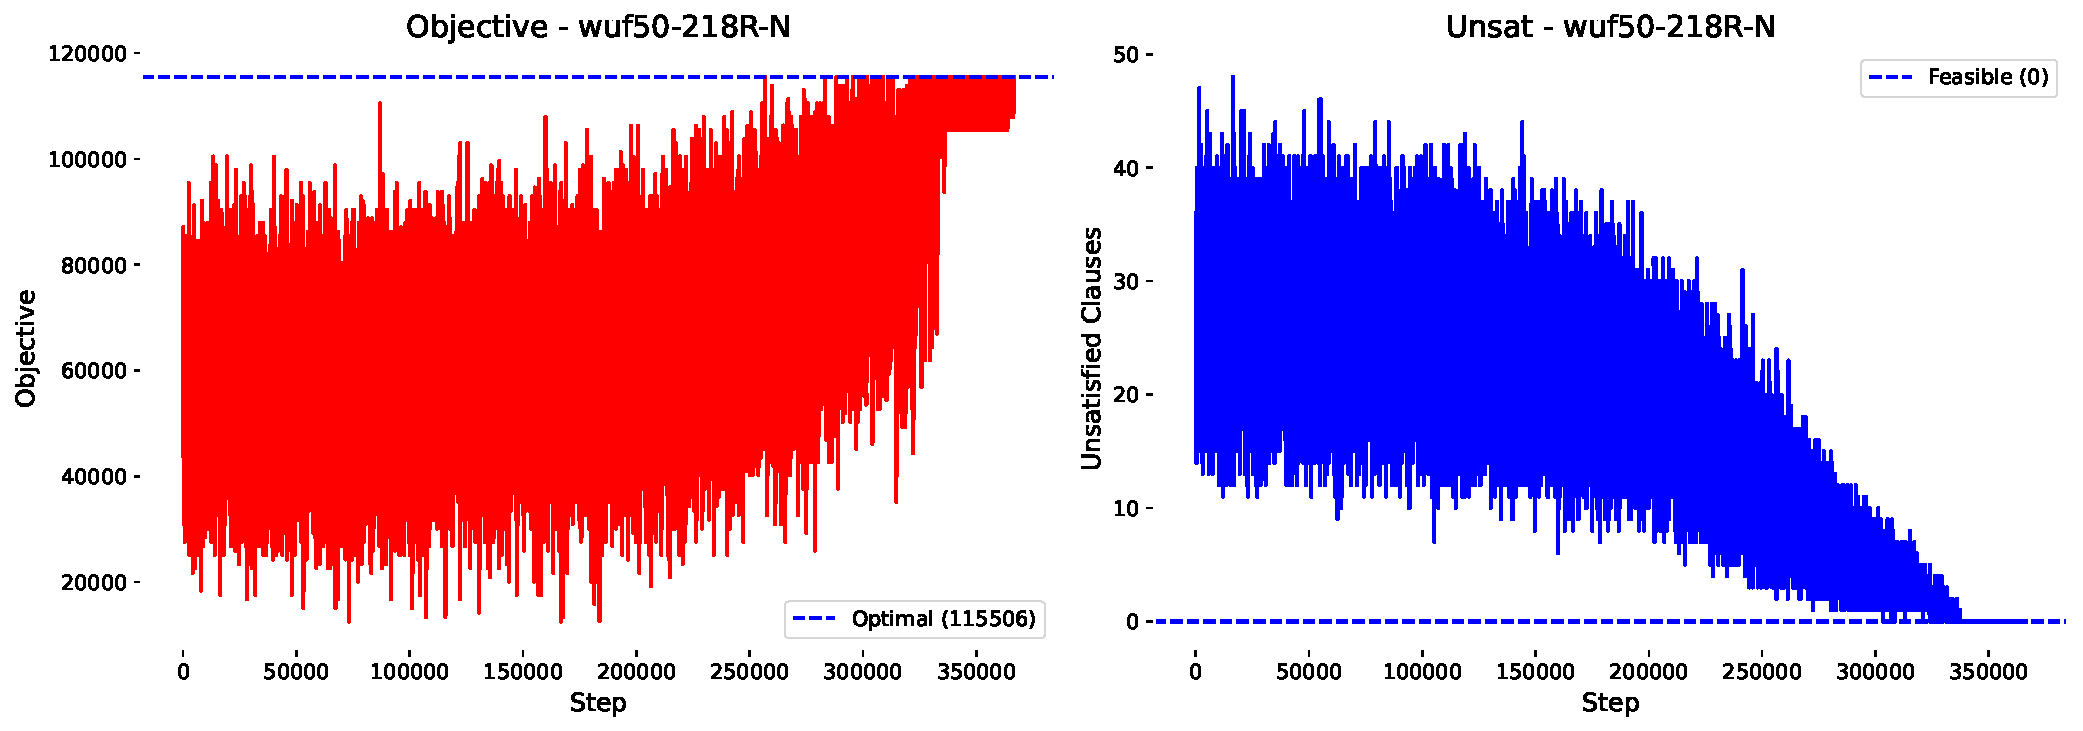
\includegraphics[width=\linewidth]{convergence_single.pdf}
        \caption{Single run convergence on wuf50-218R-N showing objective (left) and unsatisfied
        clauses (right). The decreasing variance reflects the cooling schedule.}
        \label{fig:convergence-single}
    \end{figure}

    \autoref{fig:convergence-runs} shows 10 independent runs on the same instance,
    each starting from a different random initial assignment.
    Despite different starting points, all runs converge
    to the same region and reach feasibility.
    The bottom row zooms in on the first 5000 steps,
    showing that after initial divergence the runs settle into similar trajectories.
    This consistency across random starts suggests the algorithm has iterative strength---it reliably finds good
    solutions regardless of initialization.
    Note that \autoref{fig:convergence-runs} uses a moving
    average for both objective and unsatisfied clauses, which is why the curves appear short of the
    optimal value; the raw values (shown in \autoref{fig:convergence-single}) are noisy but do reach
    the optimum.

    Note that the algorithm uses zero restarts.
    In practice, running 2--5 independent restarts
    and taking the best result would further increase the probability of finding the optimal
    assignment.

    \begin{figure}[htbp]
        \centering
        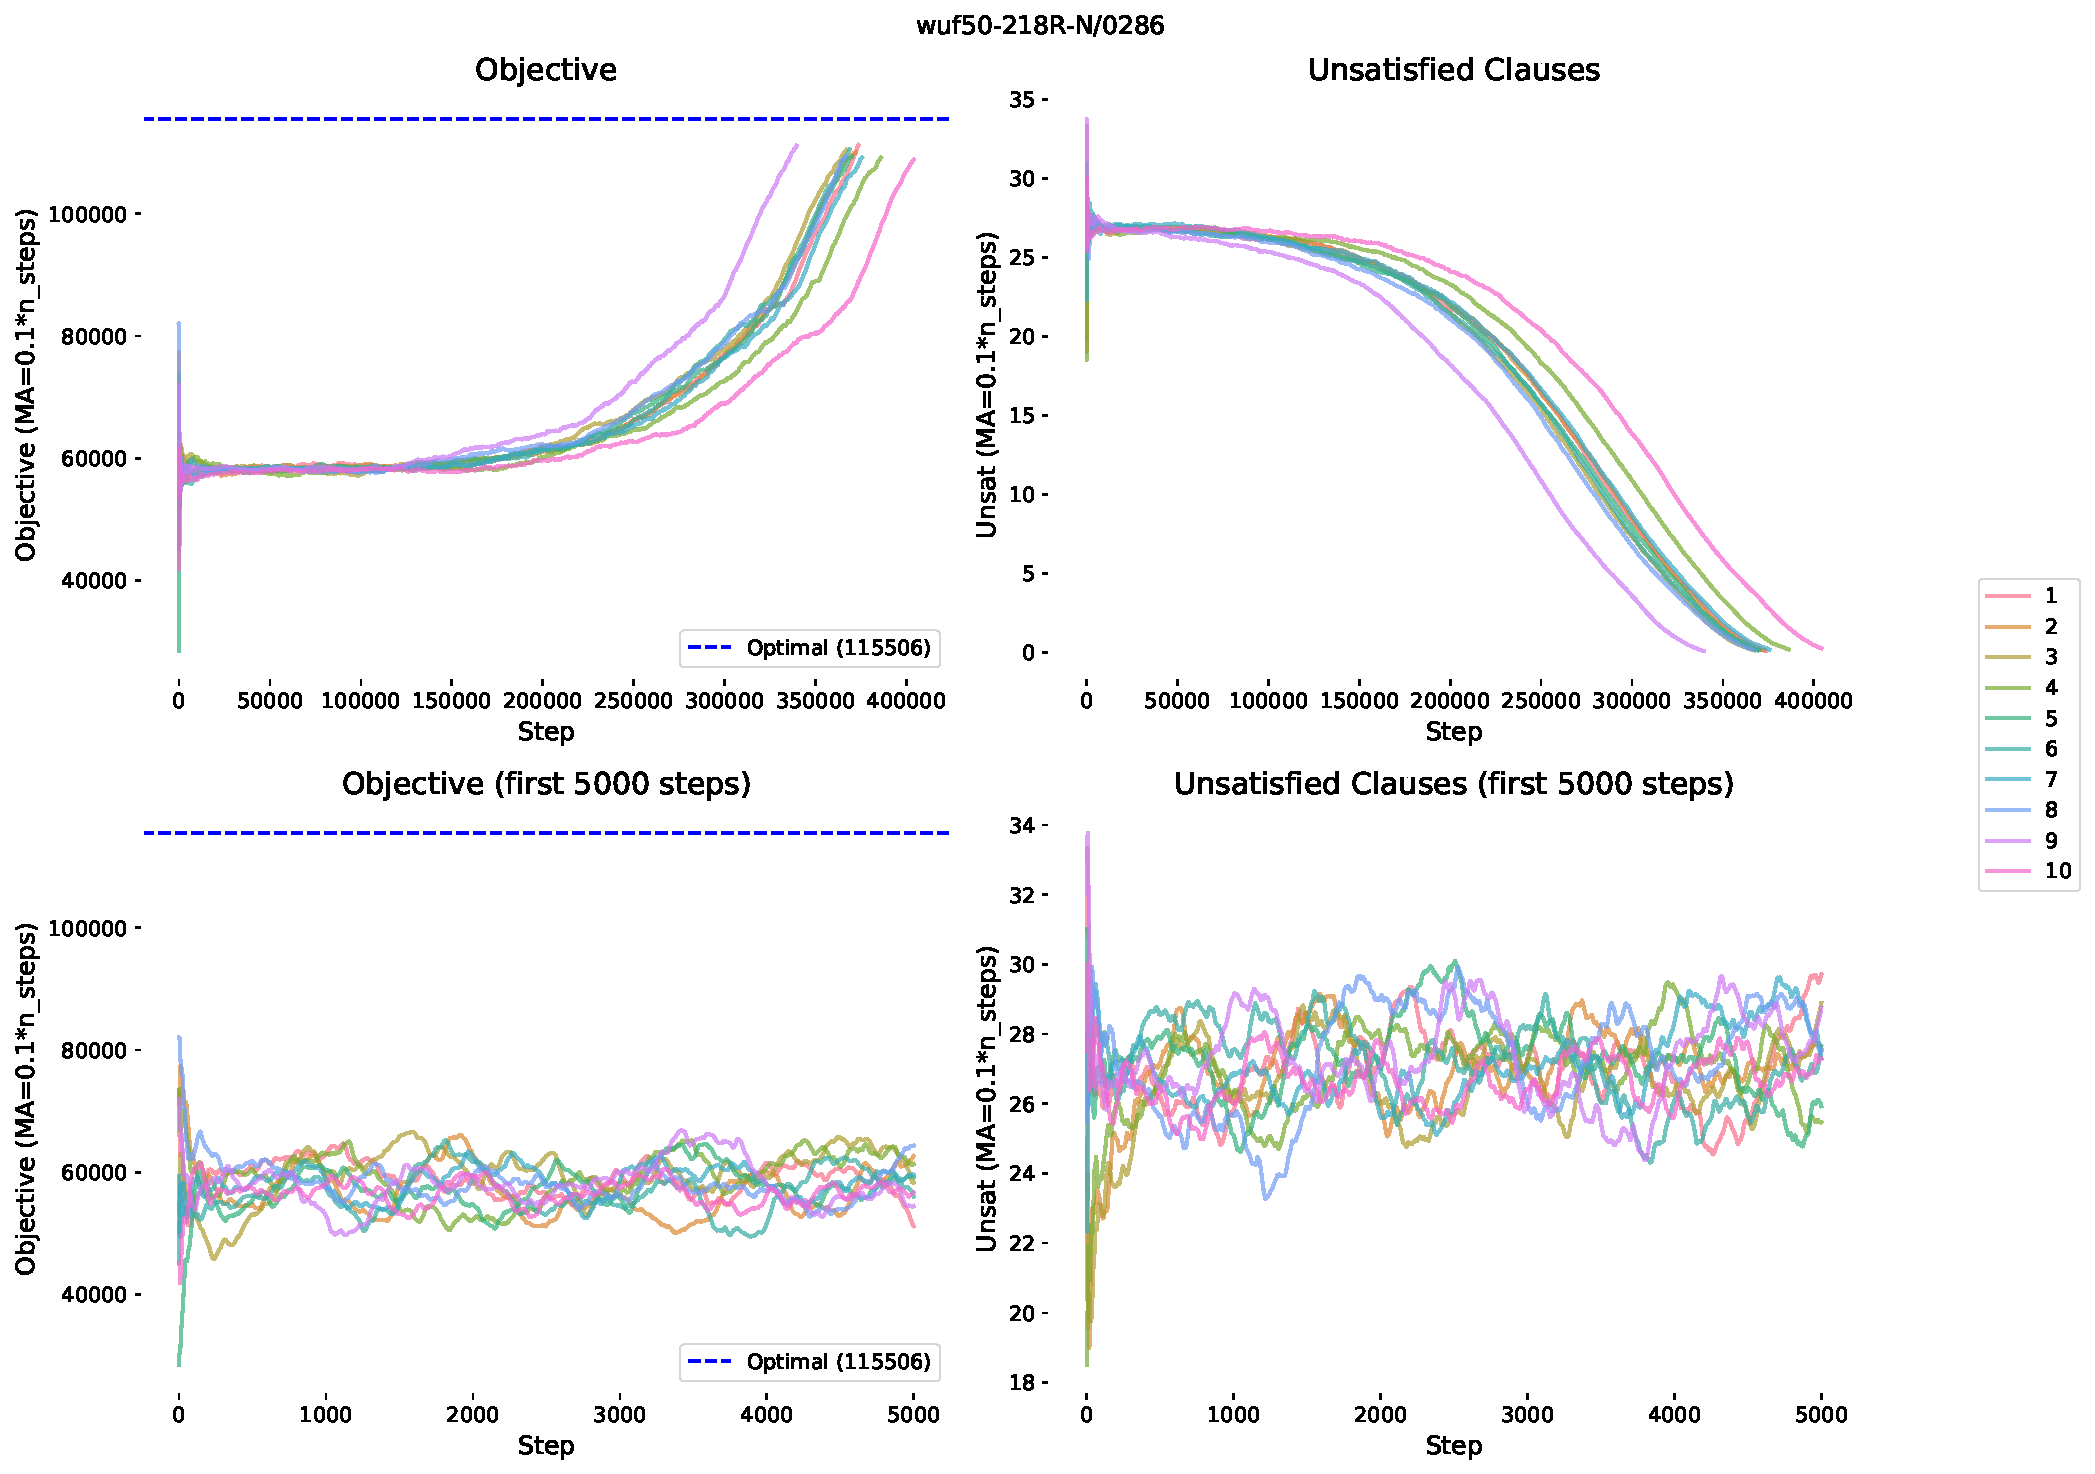
\includegraphics[width=\linewidth]{convergence_runs.pdf}
        \caption{Convergence of 10 independent runs on wuf50-218R-N/0286. Top: full run showing
        all runs reaching feasibility and converging toward optimal. Bottom: zoom on first
        5000 steps showing runs settling into similar trajectories despite random starts.}
        \label{fig:convergence-runs}
    \end{figure}

    \subsection{Final Algorithm Configuration}

    \begin{center}
        \begin{tabular}{ll}
            \toprule
            Parameter                        & Value                              \\
            \midrule
            Initial temperature              & Computed adaptively ($P_0 = 0.99$) \\
            $T_{min}/T_{max}$ ratio          & $10^{-4}$                          \\
            Number of temperature levels $K$ & 900                                \\
            Cooling rate $\alpha$            & Derived from $K$                   \\
            Equilibrium length $L_{eq}$      & $\text{clamp}(12n/a, n, 50n)$      \\
            Target accepted moves            & $\min(L_{eq}, 12n)$                \\
            \bottomrule
        \end{tabular}
    \end{center}


    \newpage


    \section{Black-Box Phase: Experimental Evaluation (IMRAD)}

    \subsection{Introduction}

    We evaluate the final simulated annealing configuration on the MWSAT problem
    to determine its effectiveness across instance sizes and characteristics.
    The heuristic should achieve comparable performance on instances with 20--50 variables
    without manual parameter adjustment.

    Research questions:
    \begin{enumerate}
        \item What is the success rate and optimality rate across instance classes?
        \item Does the adaptive mechanism provide consistent performance across instance sizes?
    \end{enumerate}

    \subsection{Methods}

    \subsubsection{Algorithm Summary}

    The simulated annealing algorithm uses a weighted energy function prioritizing feasibility
    over optimality, adaptive initial temperature based on acceptance probability, geometric
    cooling with 900 temperature levels, adaptive equilibrium length based on acceptance rate,
    and early termination when a valid solution is found and acceptance rate drops to zero.

    \subsubsection{Instance Sets}

    Instance sets from the course page: wruf36-157, wuf20-71R, wuf20-91, wuf20-91R, wuf50-218,
    and wuf50-218R. These sets were chosen because they provide reference optimal assignments,
    allowing direct comparison of solver results against known optima.

    \subsubsection{Experimental Protocol}

    To control for randomization, experiments follow a two-stage protocol.
    First, suppress randomization variance by running the solver $r = 100$ times on each instance.
    Second, suppress instance variance by aggregating over all instances in each set.
    Total: $13200 \times 100 = 1.32 \times 10^6$ solver invocations.

    \subsubsection{Metrics}

    \begin{itemize}
        \item \textbf{Solved (\%)}---percentage of runs finding a satisfying assignment.
        \item \textbf{Optimal (\%)}---percentage of runs finding the known optimal solution.
    \end{itemize}

    \subsubsection{Implementation}

    The solver is implemented in C++17.
    Batch execution uses GNU Parallel~\cite{tange_2025_18039569}
    to run one binary per instance file, where each binary performs all $r$ repetitions internally.
    This reduces parallelization overhead since individual SA runs complete quickly and spawning
    a new process per run would leave CPUs idle waiting for jobs.

    Final evaluation was performed on Metacentrum using a 32-core AMD EPYC 7543 (roughly 45 minutes).

    \subsection{Results}

    \begin{table}[htbp]
        \centering
        \caption{Final evaluation results across all instance sets.}
        \label{tab:final-results}
        \begin{tabular}{lcc}
            \toprule
            Dataset      & Solved (\%) & Optimal (\%) \\
            \midrule
            wuf20-71R-M  & 100.00      & 100.00       \\
            wuf20-71R-N  & 100.00      & 100.00       \\
            wuf20-71R-Q  & 100.00      & 99.55        \\
            wuf20-71R-R  & 100.00      & 99.55        \\
            \midrule
            wuf20-91-M   & 100.00      & 100.00       \\
            wuf20-91-N   & 100.00      & 100.00       \\
            wuf20-91-Q   & 100.00      & 100.00       \\
            wuf20-91-R   & 100.00      & 100.00       \\
            \midrule
            wuf20-91R-M  & 100.00      & 100.00       \\
            wuf20-91R-N  & 100.00      & 100.00       \\
            wuf20-91R-Q  & 100.00      & 100.00       \\
            wuf20-91R-R  & 100.00      & 100.00       \\
            \midrule
            wruf36-157-M & 100.00      & 99.99        \\
            wruf36-157-N & 100.00      & 99.99        \\
            wruf36-157-Q & 99.75       & 99.04        \\
            wruf36-157-R & 99.76       & 99.06        \\
            \midrule
            wuf50-218-M  & 99.94       & 99.56        \\
            wuf50-218-N  & 99.92       & 99.55        \\
            wuf50-218-Q  & 98.12       & 90.63        \\
            wuf50-218-R  & 98.20       & 90.59        \\
            \midrule
            wuf50-218R-M & 99.92       & 99.63        \\
            wuf50-218R-N & 99.95       & 99.61        \\
            wuf50-218R-Q & 97.46       & 89.76        \\
            wuf50-218R-R & 97.69       & 89.93        \\
            \bottomrule
        \end{tabular}
    \end{table}

    \subsection{Discussion}

    The heuristic achieves 100\% satisfiability and near-100\% optimality on 20-variable instances,
    $>$99\% satisfiability on 36 and 50-variable instances with M/N weights, and $>$97\%
    satisfiability on difficult Q/R weight distributions.
    Optimality rates remain above 89\% even on the most challenging instances.

    Performance degrades gracefully from 20 to 50 variables, demonstrating that adaptive mechanisms
    successfully adjust to instance difficulty.

    The convergence plots (\autoref{fig:convergence-single}, \autoref{fig:convergence-runs}) demonstrate
    iterative strength: the algorithm consistently improves solutions over time, with all runs
    reaching feasibility and most reaching optimality.

    \subsection{Conclusion}

    The simulated annealing heuristic with adaptive mechanisms achieves $>$97\% satisfiability
    and $>$89\% optimality across all tested instance classes (20--50 variables).
    The adaptive initial temperature, equilibrium length, and derived cooling rate enable consistent performance
    without manual parameter tuning per instance.


    \section*{Acknowledgments}

    Computational resources were provided by the e-INFRA CZ project (ID:90254),
    supported by the Ministry of Education, Youth and Sports of the Czech Republic.

    \begin{thebibliography}{9}

        \bibitem{tange_2025_18039569}
        Ole Tange.
        \textit{GNU Parallel 20251222 ('Bondi')}.
        Zenodo, December 2025.
        \url{https://doi.org/10.5281/zenodo.18039569}

        \bibitem{kop_sa_lecture}
        \textit{KOP08: Simulované ochlazování} [Lecture slides].
        NI-KOP, FIT CVUT, 2023.

    \end{thebibliography}

\end{document}
